\documentclass[11pt]{article}
\usepackage{tikz}
\usepackage{amsmath}
\usepackage{amssymb}
\usetikzlibrary{calc,intersections}
\usetikzlibrary{arrows,calc}

\begin{document}

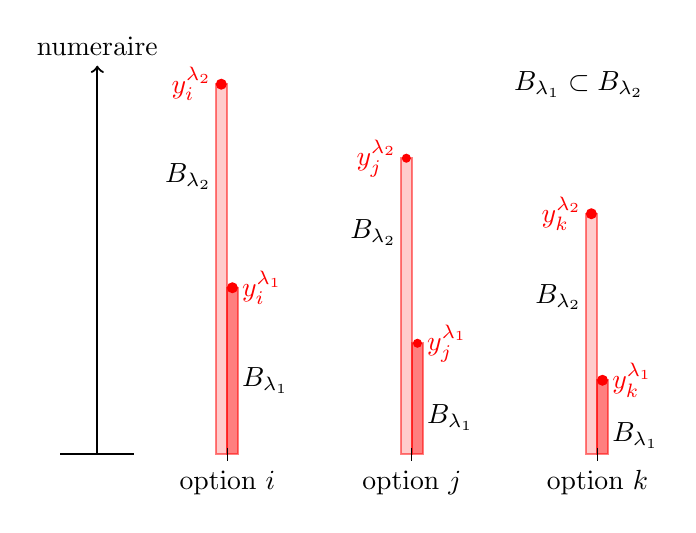
\begin{tikzpicture}[scale=2.35,domain=0:1]
    % Draw axes
    \draw [->,thick] (-0.2,0) -- (-0.2,2.1) node [above] {numeraire} ;
   \draw [-,thick]  (-0.4,0) -- (0,0);

                       \node[ black ,right] at (2,2) {$B_{\lambda_1} \subset B_{\lambda_2}$} ;

      
       \filldraw [color=red,thick,fill=red!40,semitransparent]  (0.44,2) --  (0.50,2)--(0.50,0)--(0.44,0)--cycle;
       \filldraw [color=red,thick,fill=red!100,semitransparent]  (0.50,0.9) --  (0.56,0.9)--(0.56,0)--(0.50,0)--cycle;

       \filldraw [color=red,thick,fill=red!40,semitransparent]  (1.44,1.6) --  (1.50,1.6)--(1.50,0)--(1.44,0)--cycle;
       \filldraw [color=red,thick,fill=red!100,semitransparent]  (1.50,0.6) --  (1.56,0.6)--(1.56,0)--(1.50,0)--cycle;
            
       \filldraw [color=red,thick,fill=red!40,semitransparent]  (2.44,1.3) --  (2.50,1.3)--(2.50,0)--(2.44,0)--cycle;
       \filldraw [color=red,thick,fill=red!100,semitransparent]  (2.50,0.4) --  (2.56,0.4)--(2.56,0)--(2.50,0)--cycle;
    
               \node[ black ,right] at (0.53,0.4) {$B_{\lambda_1}$} ;
              \node[ black ,right] at (1.53,0.2) {$B_{\lambda_1}$} ;
               \node[ black ,right] at (2.53,0.1) {$B_{\lambda_1}$} ;

                      \node[ black,left] at (0.47,1.5) {$B_{\lambda_2}$} ;
                      \node[ black,left] at (1.47,1.2) {$B_{\lambda_2}$} ;
                      \node[ black,left] at (2.47,0.85 ) {$B_{\lambda_2}$} ;




 
 \fill[red] (0.47,2) circle (0.85pt) node [left,color = red] {$y^{\lambda_2}_{i}$} ;
 \fill[red]  (1.47,1.6) circle (0.7pt) node [left,color = red] {$y^{\lambda_2}_{j}$} ;
 \fill[red]  (2.47,1.3) circle (0.85pt) node [left,color = red] {$y^{\lambda_2}_{k}$}  ;
 
  \fill[red] (0.53,0.9) circle (0.85pt) node [right,color = red] {$y^{\lambda_1}_{i}$} ;
 \fill[red]  (1.53,0.6) circle (0.7pt) node [right,color = red] {$y^{\lambda_1}_{j}$} ;
 \fill[red]  (2.53,0.4) circle (0.85pt) node [right,color = red] {$y^{\lambda_1}_{k}$}  ;
   
    \draw [black](0.503,1pt) -- (0.503,-1pt) node[anchor=north] {option $i$};
    \draw [black](1.5,1pt) -- (1.5,-1pt) node[anchor=north] {option $j$};
    \draw [black](2.503,1pt) -- (2.503,-1pt) node[anchor=north] {option $k$};


 
\end{tikzpicture}

\end{document}